\documentclass{scrartcl}
\usepackage[utf8]{inputenc}
\usepackage{amsmath, amsfonts,amssymb}
\usepackage{graphicx}
\usepackage{xcolor}
\usepackage[format=hang,font=small,labelfont=bf]{caption}
\usepackage{bm}
% \usepackage{algorithmicx}
% \usepackage{algorithm}
% \usepackage[noend]{algpseudocode}
% \usepackage{booktabs}
% \usepackage{mathtools}
% \usepackage{float}
% \usepackage{floatpag}
% \usepackage{comment}
% \usepackage{cases}
% \usepackage{mathtools}

%%%%%% PREAMBLE

\newtheorem{theorem}{Theorem}
\newtheorem{lemma}{Lemma}
\DeclareMathOperator*{\argmax}{arg\,max}
\DeclareMathOperator*{\argmin}{arg\,min}
\DeclareMathOperator*{\unif}{Unif}
\DeclareMathOperator*{\bin}{Bin}
\DeclareMathOperator*{\bern}{Bernoulli}
\DeclareMathOperator*{\cauchy}{Cauchy}
\DeclareMathOperator*{\logit}{logit}

\newcommand{\todo}[1]{\textcolor{red}{TODO:
    #1}\PackageWarning{TODO:}{#1!}}

\newcommand{\N}{\mathbb{N}} % naturals
\newcommand{\Q}{\mathbb{Q}} % rationals
\newcommand{\Z}{\mathbb{Z}} % integers
\newcommand{\R}{\mathbb{R}} % reals
\newcommand{\ep}{\varepsilon}
\newcommand{\expect}[1]{\operatorname{\textnormal{\textbf{E}}}\left[#1\right]}
\newcommand{\dprob}[1]{\operatorname{\textnormal{Pr}}\left(#1\right)}
\newcommand{\cprob}[1]{\operatorname{p\left(#1\right)}}
\newcommand{\mat}[1]{\bm{#1}}

\begin{document}

\section{Notation at a glance}

CAR models are frequently written with several different
parameterizations and choices in variable names. For clarity, these
are the notations used in this text.

\begin{itemize}
\item [$\mat{\phi}$:] A vector $(\phi_1,\dots, \phi_n)$ of CAR random
  variables, used as spatial random effects.
\item [$\mat{A}$:] Adjacency matrix of ``raw distance,'' i.e. the
  (projected) distance between two geocoordinates. Units in meters.
\item [$\mat{C}$:] Neighborhood matrix used by a CAR model. Some
  transformation of $\mat{A}$ which then specifies which $\phi_i$'s
  are dependent on each other.
\item [$\mat{D}$:] Diagonal matrix of degrees in $\mat{C}$,
  i.e. $d_{ii} = \sum{c_{ij}} = k_i$.
\item [$\alpha$:] A ``spatial strength'' parameter which scales the
  conditional means for each $\phi_i$. The effect of varying $\alpha$
  is quite muddy and should not be interpreted as overall magnitude
  of the spatial effects.
\item [$\tau$:] A spatial precision parameter. 
\end{itemize}

% \section{Motivation}
% \label{sec:motivation}

% Here we quickly explain the motivation behind applying CAR models,
% which generally are reserved for disease mapping over larger regions,
% in our dataset. Keeping in mind that we are primarily interested in
% the shape and extent of spatial patterns of infestation, a good place
% to start would be with clustering detection methods (Moran's I,
% permutation tests). These indicate significant clustering in our data,
% but do not help with our additional interest in how spatial proximity,
% interacting with a number of other covariates, impacts a house's risk
% of infestation. 

\section{The CAR model}
\label{sec:car-model}

The traditional Conditional Autoregressive (CAR) model specifies a
vector of random variables $\mat{\phi} = (\phi_1, \dots, \phi_n)$ over
$\R^2$, where $\phi_i$ is conditional only on $\phi_j$ from a set of neighbors
$j\in N(i)$, and $\phi_i \mid \phi_j, j\in N(i)$ is normally
distributed. That is, the CAR model is a type of Gaussian Markov
Random Field (GMRF).

GMRFs are extremely general, covering a vast number of models for
discrete spatial variation (for data over a continuous domain,
geostatistical models like kriging are preferred; for data where the
observed locations are themselves random, Poisson point processes are
the way to go) \cite{Gelfand2010}. Nowadays, I get the impression that when people say
CAR model, they mean the following specification, which is the one we
use here. For a symmetric neighborhood matrix $\mat{C}$, we write

% For our setting, we can think of $i \in\{1, \dots, n\}$ as a house in a village of size $n$ and $N(i)$ as $i$'s neighbors. Then for each house $i$, we let

\begin{equation}
  \label{eq:car1}
  \phi_i|\phi_j, j \neq i \sim N\left(\frac{\alpha \sum_{j=1}^nc_{ij}\phi_j}{\sum_{j = 1}^nc_{ij}}, \frac{1}{\tau \sum_{j = 1}^nc_{ij}}\right),
\end{equation}
where $\alpha$ is a scaling parameter for spatial dependency and
$\tau$ is a scaling precision parameter. This can
also be expressed in multivariate normal form as

\begin{equation}
  \label{eq:car2}
  \mat{\phi} \sim N(0, [\tau (\mat{D} - \alpha \mat{C})]^{-1}),
\end{equation}
where $\mat{D}$ is the diagonal matrix with
$d_{ii} = \sum_{j = 1}^nc_{ij}$, provided $\alpha$ and $\mat{C}$ are
such that the above inverse exists. If we fix $\alpha = 1$, this
special case is called the Intrinsic CAR (ICAR) model; however, since
the Laplacian $\mat{D} - \mat{C}$ is never invertable, such priors are
improper. This is still a common choice though, since when used in a
hierarchical setting the posterior is proper, and fitting can be much
faster since one can now avoid inverting a matrix every likelihood
evaluation.

The most popular choice for $\mat{C}$ is as a binary adjacency matrix
for some undirected, unweighted graph. Such graphs arise, for example,
in disease mapping studies where edges represent bordering geographic
regions.

\subsection{Use in hierarchical models}
\label{sec:use-hier-models}

The CAR model can be used to represent spatial effects in a
hierarchical setting, such as a Bayesian GLM. Recall we have binary
response data $\mat{y} = (y_1,\dots, y_n)$ indicating infestation
status of each home, and an $n \times p$ matrix of covariates
$\mat{X}$ (and intercept). We can add our CAR random variables into
the link layer, so that the data likelihood is

\begin{gather}
  \label{eq:car-glm}
  y_i \mid \mat{\phi}, \mat{\beta} \sim \bern{(r_i)}\\
  \text{logit}^{-1}(r_i) = \sum_{j = 1}^p \beta_j x_{ij} + \phi_i,
\end{gather}
where $r_i$ can be interpreted as the probability a house is infested
(the ``risk'' of house $i$). Unless stated otherwise, all
specifications used here will have non-informative $\cauchy(0, 2.5)$
priors for $\mat{\beta}$, and priors for $\mat{\phi}$ distributed
according to Eq. \eqref{eq:car2} with hyperpriors
$\alpha \sim \unif(0, 1)$ and $\tau \sim \text{Gamma}(2, 1)$.

To get a sense of how the spatial effects respond to the data, note
that the posterior
$\mat{\phi} \mid \mat{y}, \mat{\beta}, \alpha, \tau$ is also a GMRF
though no longer centered at zero. In particular, anecdotally from
other likelihoods I believe they will be shifted according to the
residuals $\mat{y} - \logit(\mat{X} \mat{\beta})$, though I haven't
found a citation nor worked this out myself for the Binomial/Bernoulli
case. This is why we can think of $\mat{\phi}$ as a smoothing
parameter; when the data comes in, each $\phi_i$ has its mean adjusted
to ``fill in'' variation not explained by the covariates, while the
neighborhood structure favors neighbors to be ``filled in'' similarly.

\todo{smoothing of $r_i$'s is valuable in of itself here because...response measurements are noisy, not all houses have all or accurate covariates, covariates are autocorrelated themselves, ... and we are also interested in the network structure which leads to good smoothing since we know little about dispersal patterns}

% These CAR priors serve as random
% effects, and can be interpreted as a smoothing parameter between
% neighbors: absent of stronger signals from $Y$, a house's risk of
% infection will be more similar to the average risk of its neighbors.

\section{A CAR model with decaying neighborhood weights}
\label{sec:decaying-weights-car}

The issue with a traditional CAR model for our setting is the need to
specify a fixed neighborhood structure. A natural choice for fixed
point data such as ours would be to let $c_{ij} = [a_{ij} < h]$, so
that all houses within a radius $h$ of $i$ are connected to
$i$. Another possibility is assume the houses lie somewhere within a
square lattice, and to consider houses neighbors if they share edges
on the grid \cite{Paciorek2013}. However, with both these scenarios
the choice of $h$ or grid size is unclear; there are few obvious
constraints such as geographic boundaries, and ecological clues such
as \textit{T. dimidiata} dispersal patterns are highly variable and
poorly understood.

A handful of authors have proposed methods for removing the assumption
of a fixed network by using a stochastic neighborhood structure and
additional model parameters \cite{Gao2019, Rodrigues2012}, but none of
these ideas have seen much application to novel datasets (though see
\cite{Whittle2020}), and several make assumptions that are not
reasonable for point data.

The model we use here can be seen as a specification of the one given
in White and Ghosh (2009), termed the stochastic neighborhood CAR
(SNCAR) model \cite{White2009}. Originally, this model assumed the
local neighborhood structure was fixed, but that houses up to an
unknown larger radius are correlated inversely with distance. We
instead are interested in the case where the radius of ``nearby
neighbors'' is unknown. We will assume all houses in the village are
connected, with the strengths of these connections decaying as a
function of distance. In contrast to the step function with
exponential decay in \cite{White2009}, our first attempt has a
sigmoidal shape:

\begin{equation}
  \label{eq:decay-func}
  c_{ij} = 1 - \frac{1}{1 + \exp(-k (a_{ij} - x_0))},
\end{equation}
where $k$ and $x_0$ are respectively shape and location
parameters. The motivation here is to approximate the binary structure
assumed in a traditional CAR model, but where the cutoff radius is
unknown and has some noise. With some simplifying, we can then write
our $\mat{C}$ matrix as

\begin{equation}
  \label{eq:decay-mat1}
  \mat{C}(k, x_0, \mat{A}) = (1 + \exp(k (\mat{A} + x_0)))^{-1}.
\end{equation}

We update the matrix $\mat{D}(k, x_0, \mat{A})$ accordingly. We can
now simply use these new transformations when computing
Eq. \eqref{eq:car2}, although care must be taken to ensure the
resulting precision matrix is still positive definite. The resulting
priors $\mat{\phi} \mid x_0, k$ can be used in our hierarchical setup
in exactly the same way.

To complete the description of the model we will be using here, we use
the same hyperpriors on $\beta$, $\alpha$, $\tau$ as before. We use
uniform priors on $x_0$ and $k$, although an appropriate upper bound
on these priors is unclear. % We will discuss this in more detail in
% Section \todo{}.

% which we can For simplicity, we will rewrite 

% \begin{gather}
%   \label{eq:decay-car}
%   \mat{\phi} \sim N(0, [\tau (\mat{D} - \alpha \mat{C}())]^{-1})
% \end{gather}

\section{Comparison Study}
\label{sec:simulation-study}

We now present a simple comparison study between a traditional CAR
model and two stochastic neighborhood CAR models with decaying
weights. The first uses the sigmoidal decay function described above,
while the second uses a exponential step function more reminiscent of
the original SNCAR model:

\begin{equation}
  \label{eq:decay-mat2}
  \mat{C}(k, x_0, \mat{A}) =
  \begin{cases}
    1 & \mat{A} \leq x_0 + 1\\
    (\mat{A} - x_0)^{-k} & \text{otherwise.}
  \end{cases}
\end{equation}

See Figure \ref{fig:fig1} for examples of these two functions. A nice
property of both is that they are both equal to a binary neighborhood
matrix with cutoff radius $x_0$ as $k \rightarrow\infty$.

\begin{figure}
  \centering
  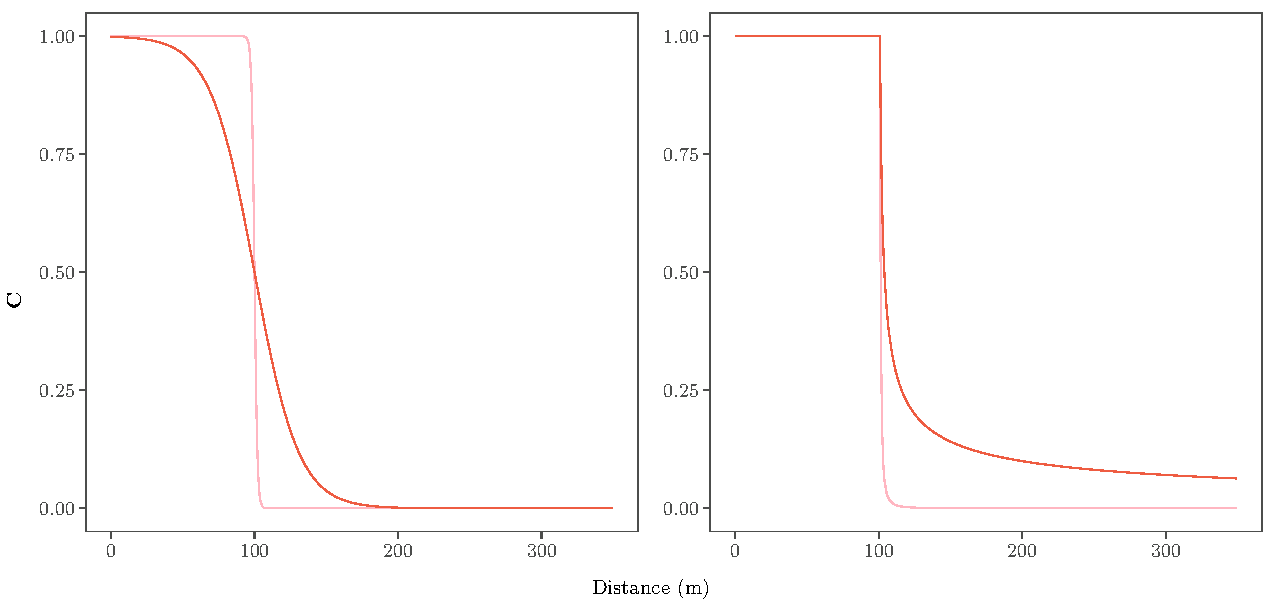
\includegraphics[width=.75\linewidth]{fig1}
  \caption{Left: Eq. \eqref{eq:decay-mat1} with $x_0 = 100$ and
    $k = 0.065$ (red), $k = 1$ (pink). Right:
    Eq. \eqref{eq:decay-mat2} with $x_0 = 100$ and $k = 0.5$ (red),
    $k = 2$ (pink).}
  \label{fig:fig1}
\end{figure}

\subsection{Data Preparation}
\label{sec:spatial-data}

We use the smallest of the five villages in our dataset (Paternito),
with all 27 covariates. 
% \todo{may want to explain contrast scheme
%   later}.
To keep the data consistent across all models, we removed
several highly isolated houses since the traditional CAR model cannot
account for these for any reasonable neighborhood radius (also, the
decaying weight models will also struggle to sample from these houses
without special considerations). Thus, we are left with a total of 96
houses, 35 of which are infested.

\subsection{Prior Distribution Results}
\label{sec:prior-distr-results}

To begin analyzing the impact of various weight matrices in the CAR
model, we first focus on the behavior of the prior for
$\mat{\phi}$. As noted above, the joint posterior for $\mat{\phi}$ can
look quite different from the prior; however, high-level observations
about the covariance structure in Eq. \eqref{eq:car2} tend to transfer
over to the posterior \cite{Assuncao2009}.

First, we examine the (Pearson) correlation between $\phi_i$ and
$\phi_j$ for all possible pairs. Since the mean of each of the priors
is 0, we have
$\text{Corr}(\phi_i, \phi_j) = \expect{\phi_i \phi_j} /
(\sigma(\phi_i) \sigma(\phi_j)) = \text{Cov}(\phi_i, \phi_j) /
(\sigma(\phi_i) \sigma(\phi_j))$, where $\sigma$ is the standard
deviation. So, we can obtain the pairwise correlation directly by
plugging in our data locations and computing the covariance matrix
given in Eq. \eqref{eq:car2}.

Figure \ref{fig:fig2} shows the correlation between all pairs within
800m as a function of distance, for a variety of neighborhood matrices
$\mat{C}$. We used the traditional CAR model with a cutoff radius of
100, along with our logistic decaying weights matrix (LCAR) and
exponential decaying weights matrix (ECAR), each with $x_0 = 100$ and
two different choices of $k$. We make some general observations:

\begin{itemize}
\item In all models, for a fixed distance there is large variation in
  the correlation. This occurs from variability in higher-order paths
  between pairs \cite{Assuncao2009}.
\item All models appear very similar when $k$ is set to a high enough
  value, though $k$ scales differently between LCAR and ECAR. When $k$
  is too low, overall correlation is much lower.
\item With the traditional CAR matrix, there is a clear region where
  correlations are either reasonably high, or exactly zero. This is
  presumably because at these distances, some points will end up in
  different connected components, so it makes sense that this does not
  appear in the decaying weights models.
\end{itemize}

Second, we plot the variance of each $\phi_i$ (i.e. the diagonal of
the joint covariance matrix) as a function of $\alpha\in(-1, 1)$ in
Figure \ref{fig:fig3}. This range for $\alpha$ was chosen to ensure
the precision matrix is invertable (though a wider range for $\alpha$
is entirely plausible, this is rarely done in practice). We plot each
$\phi_i$ as a separate line, and color each line according $i$'s
degree (i.e. $\mat{D}_{ii}$). For the traditional CAR model, notice
that variance is highest when $\alpha$ approaches both -1 and
1. Additionally, note that variance does not increase at the same rate
for all locations, as seen by the amount of line ``crossings.'' Both
these nonintuitive results are common in CAR models, and have to do
with the relative number of higher-order interactions
\cite{Assuncao2009}. However, with both decaying weights matrices,
variance is strictly monotone increase in $\alpha$, and the number of
line crossings appear much lower.

In summary, these preliminary results show the decaying weights
matrices, for the right choice of $k$, can have several potentially
desirable differences over a traditional binary neighborhood
matrix. Further inspection of these priors is warranted to better
understand the effect of different combinations of $\alpha$, $x_0$,
and $k$.

\begin{figure}
  \centering
  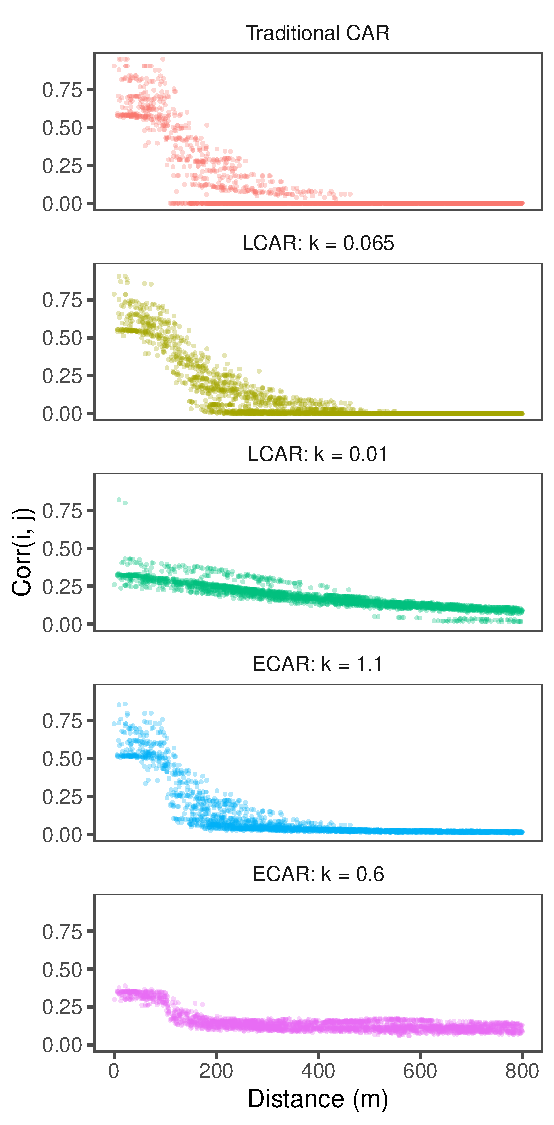
\includegraphics[width=.5\linewidth]{fig2}
  \caption{Correlation between all pairs $(\phi_i, \phi_j)$. For each
    model, we used $x_0 = 100$ and $\alpha = 0.95$. Pairs farther
    than 800m were removed.}
  \label{fig:fig2}
\end{figure}

\begin{figure}
  \centering
  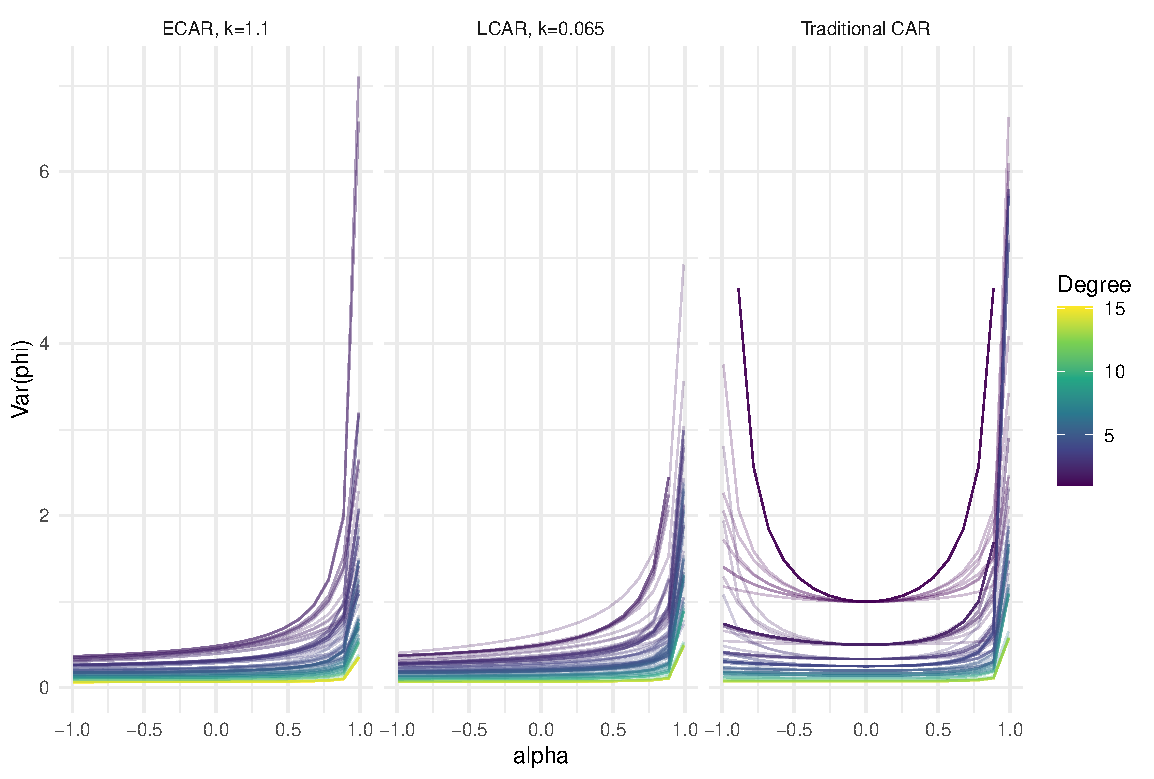
\includegraphics[width=\linewidth]{fig3}
  \caption{Variance of spatial effect priors as $\alpha$ changes. For
    all three models, we set cutoff $x_0 = 100$. Each line represents
    a separate $\phi_i$, while the color of each line corresponds to
    house $i$'s degree in the corresponding weight matrix. Points with
    variance greater than $7.5$ were removed.}
  \label{fig:fig3}
\end{figure}

\subsection{Posterior Results}
\label{sec:posterior-results}

In Section \ref{sec:prior-distr-results}, we demonstrated that the
right choice of decaying weights matrix for the prior $\mat{\phi}$ can
lead to several potential useful differences compared to a binary
neighborhood matrix. Of course, what we really care about is whether
we can estimate a reasonable $\mat{C}(k, x_0, A)$ from the data, and
if these prior differences carry over to meaningful advantages in the
posterior.

To begin answering these questions, we began by fitting two models
using a traditional neighborhood matrix and the LCAR matrix from
Eq. \eqref{eq:decay-mat1}, respectively. For the latter, we use
uniform priors for $k$ and $x_0$, but with conservative ranges based
on observations from Section \ref{sec:prior-distr-results}. We make
this simplifying assumption for now to avoid situations where the
variance on $\mat{\phi}$ explodes. For all models we obtained 20,000
posterior draws plus 8,000 warm-up iterations.

\todo{looking at the surface of spatial effects only, or surface of
  prob that $\phi_i$ is greater than $\bar{mat{\phi}}$, also has use
  for answering: even if I improve this house significantly, is it
  still at risk if I fail to improve houses around it?}

\subsubsection{Diagnosing the LCAR Posterior}
\label{sec:diagn-lcar-post}

We begin by examining the quality and nature of the posterior
fit. While there was no divergences and the chains mixed well, in all
the CAR models Stan reports the posterior may not have fully
converged. Figure \ref{fig:pairs-full} shows a pairs plot for the key
spatial parameters. We find several promising features, most
prominently that $x_0$ has shrunk to strongly indicate a very
reasonable cutoff radius.

\begin{figure}
  \centering
  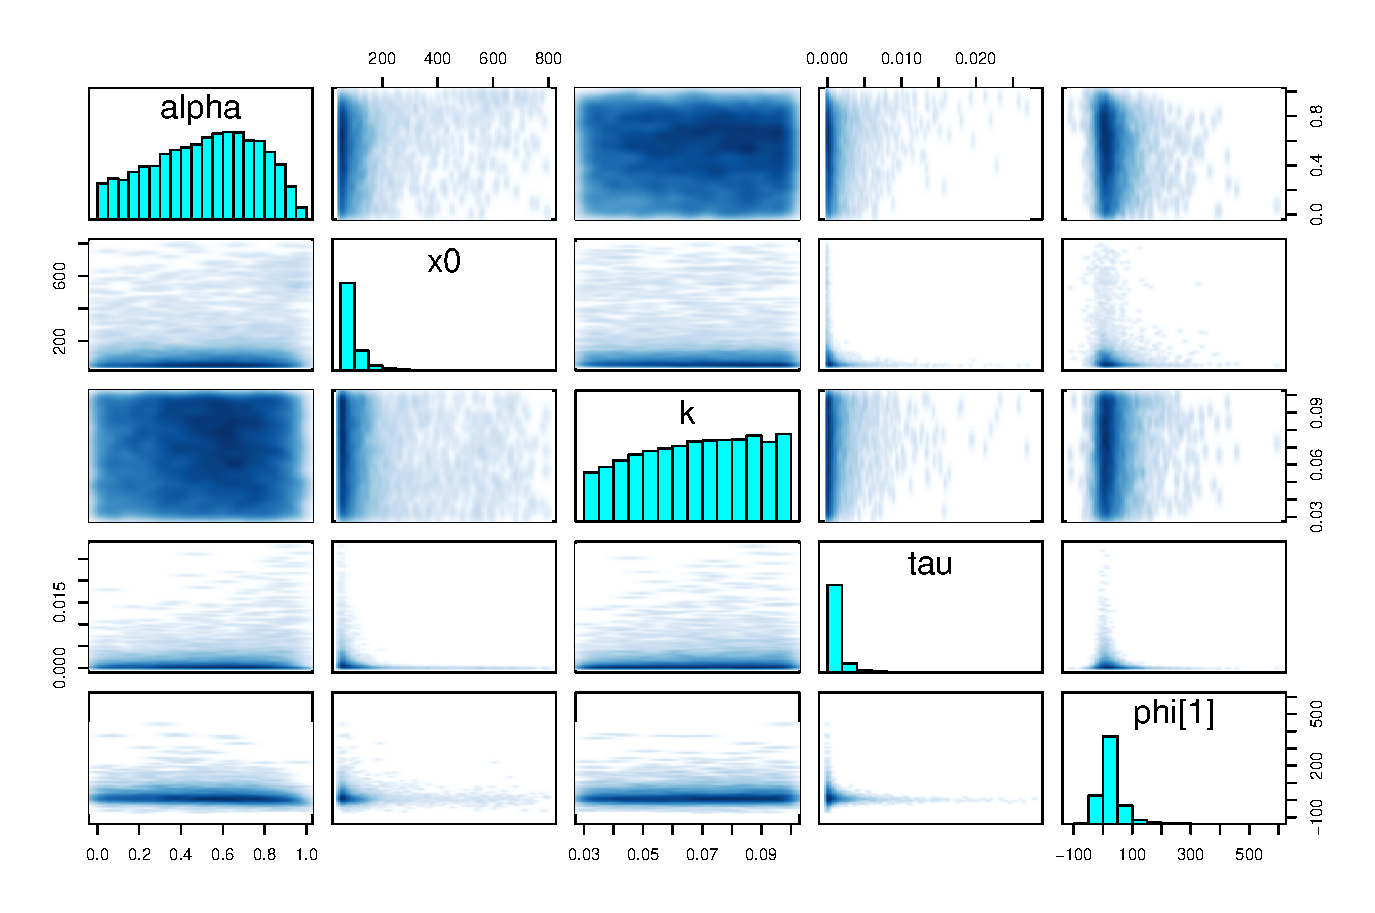
\includegraphics[width=.9\linewidth]{pairs-full}
  \caption{Posterior pairs plot using the LCAR neighborhood matrix
    with both $\alpha$ and $k$ free. The diagonal represents the
    marginal posterior for each parameter, while off diagonal shows
    interactions.}
  \label{fig:pairs-full}
\end{figure}

\begin{figure}
  \centering
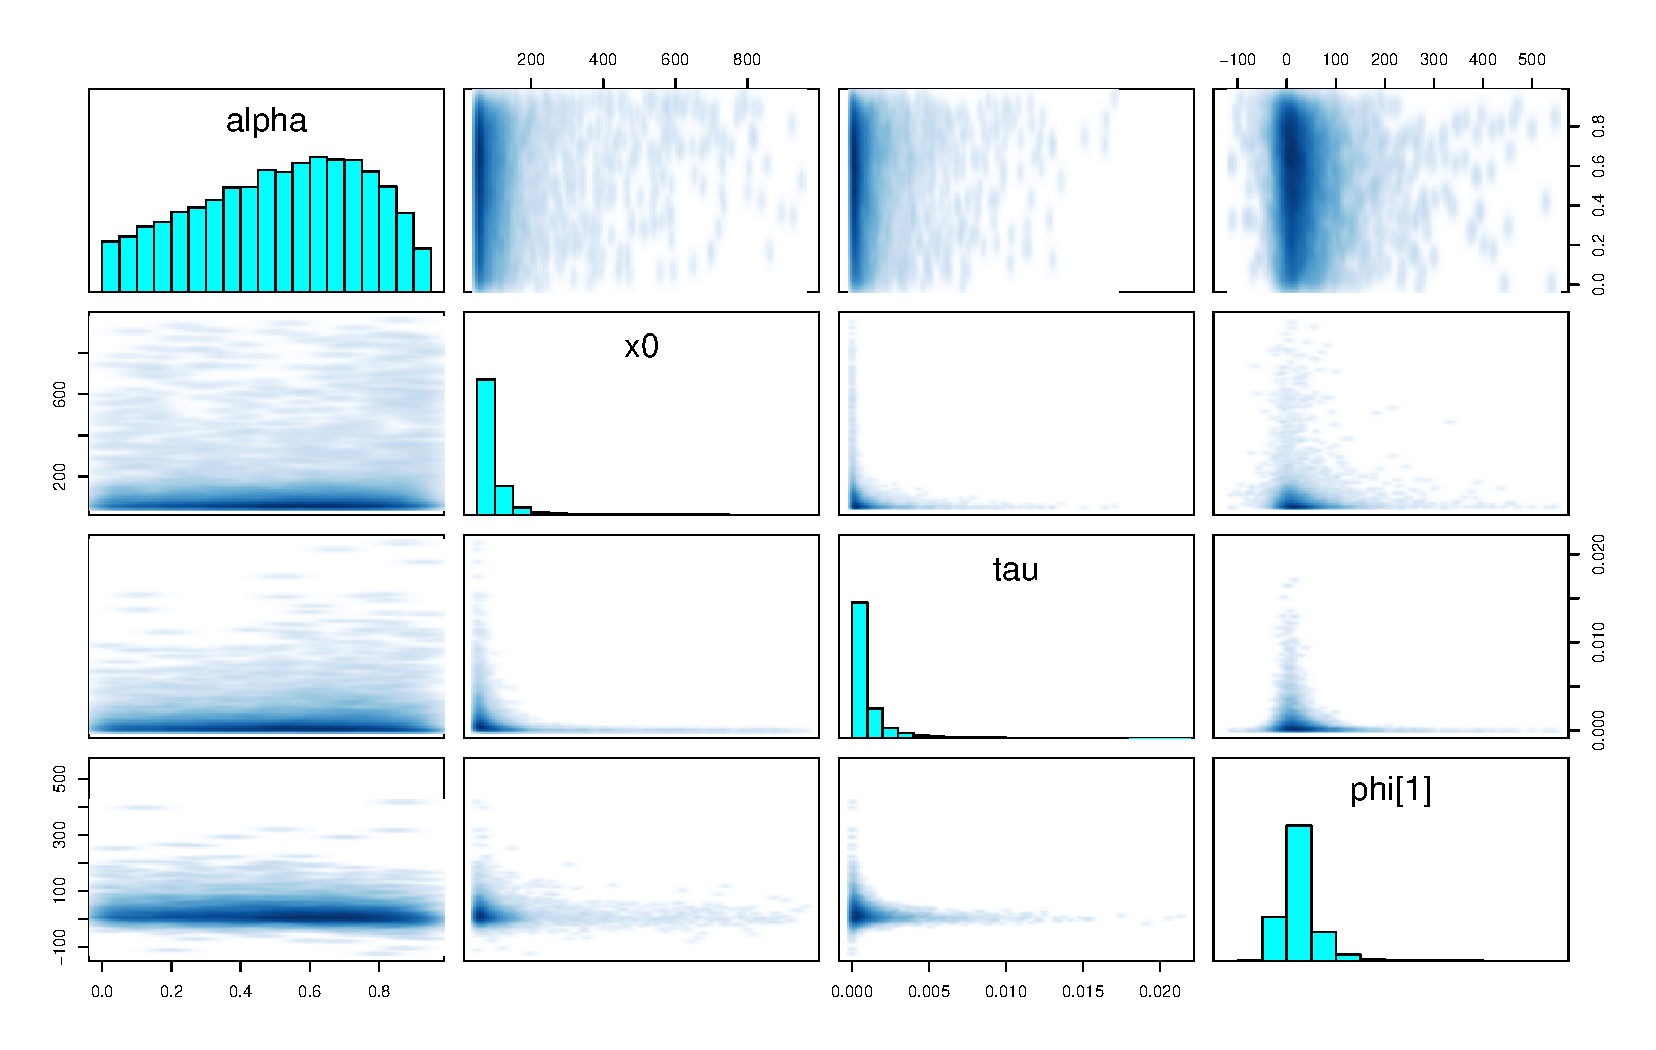
\includegraphics[width=.9\linewidth]{pairs-k-fixed}
  \caption{Posterior pairs plot using the LCAR neighborhood matrix
    with $k$ fixed to be $0.065$.}
  \label{fig:pairs-full}
\end{figure}

\begin{figure}
  \centering
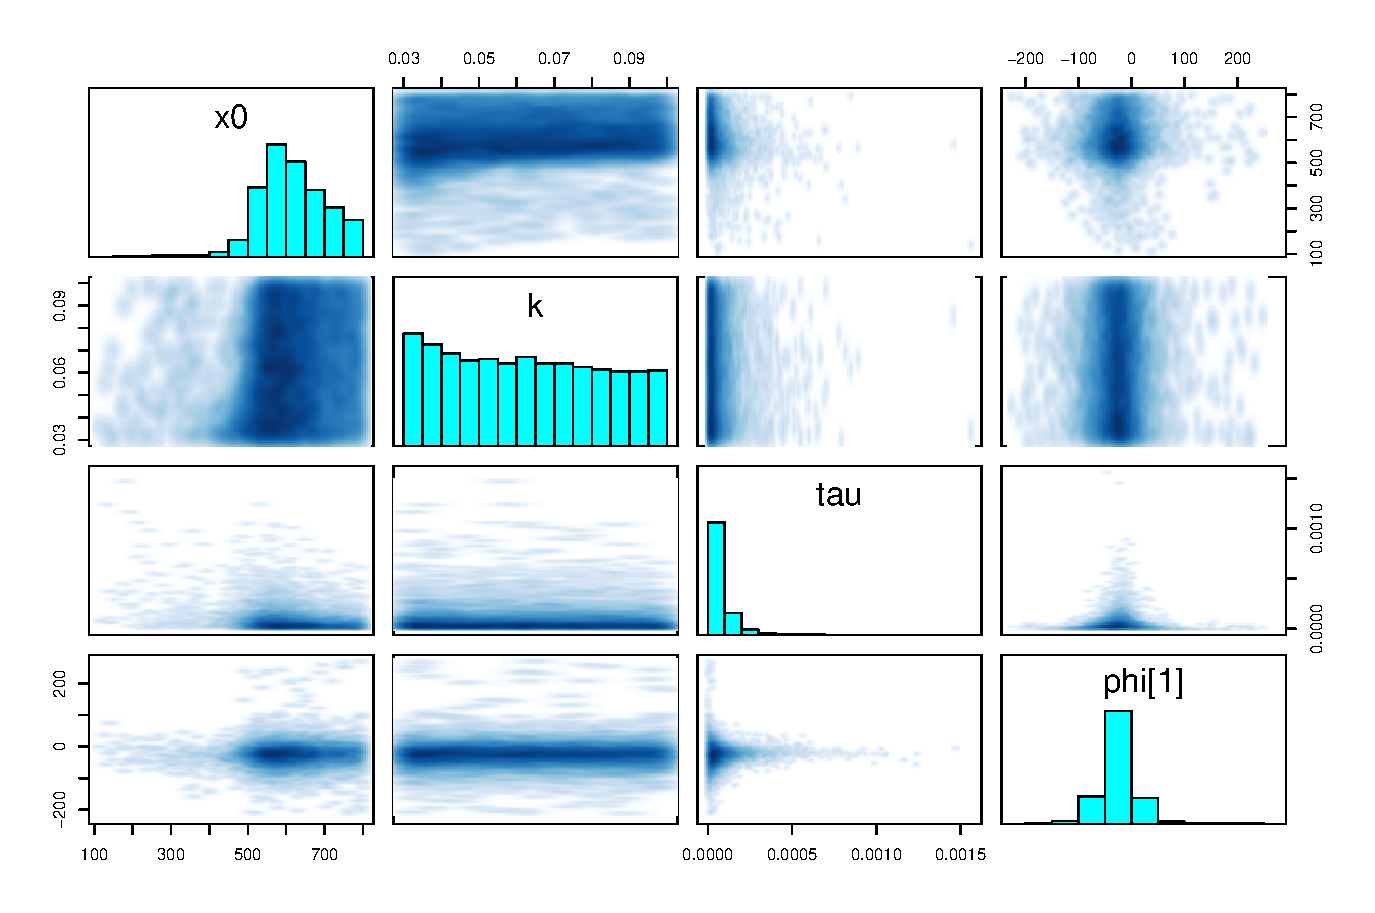
\includegraphics[width=.9\linewidth]{pairs-alpha-fixed}
\caption{Posterior pairs plot using the LCAR neighborhood matrix with
  $\alpha$ fixed to be $0.999$, so as to closely imitate an ICAR
  prior.}
  \label{fig:pairs-full}
\end{figure}

\begin{figure}
  \centering
  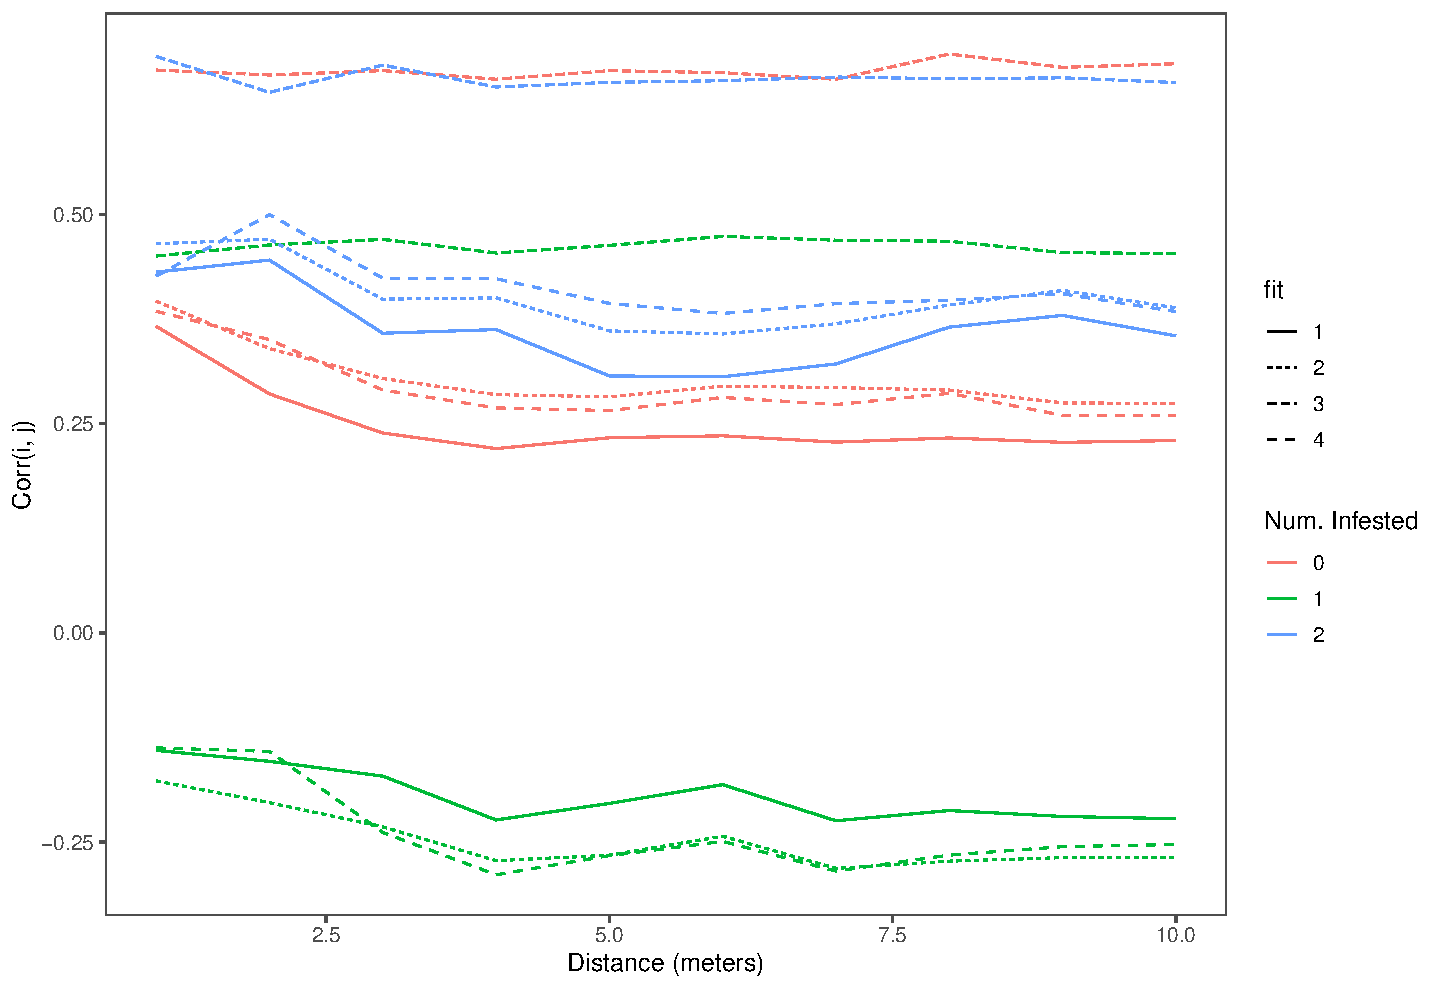
\includegraphics[width=\linewidth]{mean-corr-all}
  \caption{Average correlation by binned distances of 50m. Color
    indicates the number of infested houses in the pair, while dash
    type indicates which model was used.}
  \label{fig:mean-corr-all}
\end{figure}

% \section{Questions and remaining work}
% \label{sec:quest-rema-work}

% \begin{itemize}
% \item One feature of the traditional CAR model is that the correlation
%   $\rho(\phi_i, \phi_j)$ generally decreases as $i$'s degree
%   increases. However, this seems unreasonable in our model for
%   $c_{ij} \leq 1$; why would a house with a single, far away neighbor
%   be more correlated than a house with a single, very close neighbor?
% \end{itemize}

\bibliographystyle{abbrv}
\bibliography{C:/Users/brendandaisy/Documents/citations/chagas}

\end{document}


%%% Local Variables:
%%% mode: latex
%%% TeX-master: t
%%% End:
